% Options for packages loaded elsewhere
\PassOptionsToPackage{unicode}{hyperref}
\PassOptionsToPackage{hyphens}{url}
\PassOptionsToPackage{dvipsnames,svgnames,x11names}{xcolor}
%
\documentclass[journal=asbcd6,manuscript=article,layout=traditional]{achemso}
\usepackage[version=3]{mhchem}
\newcommand*\mycommand[1]{\texttt{\emph{#1}}}



\usepackage{amsmath,amssymb}
\usepackage{iftex}
\ifPDFTeX
  \usepackage[T1]{fontenc}
  \usepackage[utf8]{inputenc}
  \usepackage{textcomp} % provide euro and other symbols
\else % if luatex or xetex
  \usepackage{unicode-math}
  \defaultfontfeatures{Scale=MatchLowercase}
  \defaultfontfeatures[\rmfamily]{Ligatures=TeX,Scale=1}
\fi
\usepackage{lmodern}
\ifPDFTeX\else  
    % xetex/luatex font selection
\fi
% Use upquote if available, for straight quotes in verbatim environments
\IfFileExists{upquote.sty}{\usepackage{upquote}}{}
\IfFileExists{microtype.sty}{% use microtype if available
  \usepackage[]{microtype}
  \UseMicrotypeSet[protrusion]{basicmath} % disable protrusion for tt fonts
}{}
\makeatletter
\@ifundefined{KOMAClassName}{% if non-KOMA class
  \IfFileExists{parskip.sty}{%
    \usepackage{parskip}
  }{% else
    \setlength{\parindent}{0pt}
    \setlength{\parskip}{6pt plus 2pt minus 1pt}}
}{% if KOMA class
  \KOMAoptions{parskip=half}}
\makeatother
\usepackage{xcolor}
\setlength{\emergencystretch}{3em} % prevent overfull lines
\setcounter{secnumdepth}{5}
% Make \paragraph and \subparagraph free-standing
\ifx\paragraph\undefined\else
  \let\oldparagraph\paragraph
  \renewcommand{\paragraph}[1]{\oldparagraph{#1}\mbox{}}
\fi
\ifx\subparagraph\undefined\else
  \let\oldsubparagraph\subparagraph
  \renewcommand{\subparagraph}[1]{\oldsubparagraph{#1}\mbox{}}
\fi


\providecommand{\tightlist}{%
  \setlength{\itemsep}{0pt}\setlength{\parskip}{0pt}}\usepackage{longtable,booktabs,array}
\usepackage{calc} % for calculating minipage widths
% Correct order of tables after \paragraph or \subparagraph
\usepackage{etoolbox}
\makeatletter
\patchcmd\longtable{\par}{\if@noskipsec\mbox{}\fi\par}{}{}
\makeatother
% Allow footnotes in longtable head/foot
\IfFileExists{footnotehyper.sty}{\usepackage{footnotehyper}}{\usepackage{footnote}}
\makesavenoteenv{longtable}
\usepackage{graphicx}
\makeatletter
\def\maxwidth{\ifdim\Gin@nat@width>\linewidth\linewidth\else\Gin@nat@width\fi}
\def\maxheight{\ifdim\Gin@nat@height>\textheight\textheight\else\Gin@nat@height\fi}
\makeatother
% Scale images if necessary, so that they will not overflow the page
% margins by default, and it is still possible to overwrite the defaults
% using explicit options in \includegraphics[width, height, ...]{}
\setkeys{Gin}{width=\maxwidth,height=\maxheight,keepaspectratio}
% Set default figure placement to htbp
\makeatletter
\def\fps@figure{htbp}
\makeatother

\makeatletter
\makeatother
\makeatletter
\makeatother
\makeatletter
\@ifpackageloaded{caption}{}{\usepackage{caption}}
\AtBeginDocument{%
\ifdefined\contentsname
  \renewcommand*\contentsname{Table of contents}
\else
  \newcommand\contentsname{Table of contents}
\fi
\ifdefined\listfigurename
  \renewcommand*\listfigurename{List of Figures}
\else
  \newcommand\listfigurename{List of Figures}
\fi
\ifdefined\listtablename
  \renewcommand*\listtablename{List of Tables}
\else
  \newcommand\listtablename{List of Tables}
\fi
\ifdefined\figurename
  \renewcommand*\figurename{Figure}
\else
  \newcommand\figurename{Figure}
\fi
\ifdefined\tablename
  \renewcommand*\tablename{Table}
\else
  \newcommand\tablename{Table}
\fi
}
\@ifpackageloaded{float}{}{\usepackage{float}}
\floatstyle{ruled}
\@ifundefined{c@chapter}{\newfloat{codelisting}{h}{lop}}{\newfloat{codelisting}{h}{lop}[chapter]}
\floatname{codelisting}{Listing}
\newcommand*\listoflistings{\listof{codelisting}{List of Listings}}
\makeatother
\makeatletter
\@ifpackageloaded{caption}{}{\usepackage{caption}}
\@ifpackageloaded{subcaption}{}{\usepackage{subcaption}}
\makeatother
\makeatletter
\@ifpackageloaded{tcolorbox}{}{\usepackage[skins,breakable]{tcolorbox}}
\makeatother
\makeatletter
\@ifundefined{shadecolor}{\definecolor{shadecolor}{rgb}{.97, .97, .97}}
\makeatother
\makeatletter
\makeatother
\makeatletter
\makeatother
\ifLuaTeX
  \usepackage{selnolig}  % disable illegal ligatures
\fi
\IfFileExists{bookmark.sty}{\usepackage{bookmark}}{\usepackage{hyperref}}
\IfFileExists{xurl.sty}{\usepackage{xurl}}{} % add URL line breaks if available
\urlstyle{same} % disable monospaced font for URLs
\hypersetup{
  pdftitle={Bayesian regression facilitates quantitative modelling of cell metabolism},
  pdfauthor={Teddy Groves; Nicholas Luke Cowie; Lars Keld Nielsen},
  pdfkeywords={Bayesian inference, kinetic models of cell metabolism},
  colorlinks=true,
  linkcolor={blue},
  filecolor={Maroon},
  citecolor={Blue},
  urlcolor={Blue},
  pdfcreator={LaTeX via pandoc}}

\author{Teddy Groves}
\affiliation{DTU Biosustain, DTU, Kongens Lyngby, Denmark}

\altaffiliation{These authors contributed equally to this research.}

\email{tedgro@biosustain.dtu.dk}
\author{Nicholas Luke Cowie}
\affiliation{DTU Biosustain, DTU, Kongens Lyngby, Denmark}

\altaffiliation{These authors contributed equally to this research.}

\author{Lars Keld Nielsen}
\affiliation{Australian Institute for Bioengineering and Nanotechnology
(AIBN), The University of Queensland, St Lucia, Australia}
\affiliation{DTU Biosustain, DTU, Kongens Lyngby, Denmark}




\keywords{Bayesian inference, kinetic models of cell metabolism}

\title[]{Bayesian regression facilitates quantitative modelling of cell
metabolism}
\makeatletter
\begin{document}
\maketitle
\begin{abstract}
This paper presents Maud, a command-line application that implements
Bayesian statistical inference for kinetic models of biochemical
metabolic reaction networks. Maud takes into account quantitative
information from omics experiments and background knowledge, as well as
structural information about kinetic mechanisms, regulatory interactions
and enzyme knockouts. Our paper reviews the existing options in this
area, presents a case study illustrating how Maud can be used to analyse
a metabolic network and explains the biological, statistical and
computational design decisions underpinning Maud.
\end{abstract}
\ifdefined\Shaded\renewenvironment{Shaded}{\begin{tcolorbox}[sharp corners, boxrule=0pt, enhanced, breakable, frame hidden, borderline west={3pt}{0pt}{shadecolor}, interior hidden]}{\end{tcolorbox}}\fi

\hypertarget{introduction}{%
\section{Introduction}\label{introduction}}

A kinetic model of cellular metabolism aims to express what is known
about a cellular process in the form of an \emph{in silico}
representation of the underlying network of chemical reactions. Kinetic
models can be used to improve production of target molecules, determine
regulatory networks \citep{christodoulou_reserve_2018} and identify
potential drug targets
\citep{deberardinis_fundamentals_2016, Liberti2017}. However, the use of
kinetic models in practice is hindered by their dependence on noisy and
uncertain information sources. Quantitative in vivo measurements of
chemical abundances, and in vitro measurements relating to kinetic
parameters, both contain vital information but are notoriously
inaccurate (REFERENCES). Practically useful kinetic modelling therefore
requires a principled statistical approach that encompasses multiple
possible model parameterisations.

Bayesian statistical inference can combine the structural information
implicit in kinetic models with knowledge about metabolic parameters and
information from omics measurements
\citep{saa_construction_2016, gopalakrishnan_k-fit_2020}. However,
kinetic models pose serious computational challenges for Bayesian
inference \citep{gutenkunst_2007, raue_identifiability_2010}.

The scope of a kinetic model is defined by a stoichiometric matrix,
\(S\), in which rows represent metabolites, columns represent reactions,
and matrix elements \(s_{ij}\) represent the stoichiometric coefficient
of metabolite \(i\) in reaction \(j\). The change in metabolite
concentrations is:

\begin{equation}\label{eq-1}
\frac{dC}{dt} = S\cdot v - \mu\cdot C 
\end{equation}

In equation \eqref{eq-1}, C represents a vector of metabolite
concentrations, \(v\) is a vector of reaction rates, and \(\mu\) is the
growth rate. The second term represents the dilution due to cell growth.

In a kinetic model, the rates, \(v\), are expressed as a function of the
enzyme concentrations, \(E\), the metabolite concentrations, \(C\), and
a set of parameters, \(\theta\) as shown in equation \eqref{eq-2}

\begin{equation}\label{eq-2}
v = f(C, E, \theta)
\end{equation}

The parameters must include sufficient boundary concentrations and
fluxes to solve equation \eqref{eq-1}.

It is common to assume pseudo-steady state for metabolites, i.e., the
rate of fluxes towards any metabolite is much greater than the rate of
change in concentration, \(𝑣 \gg \frac{𝑑𝐶}{𝑑𝑡}\). Moreover, the dilution
effect is assumed minimal, \(\mu\cdot C \ll \vec{v}\) (true unless the
concentration is very high). Finally, the enzyme concentration is
assumed constant for the period considered and hence part of the
parameters.

Given these assumptions and a set of values for \theta, a set of steady
state metabolite concentrations and fluxes can be found by solving for
\(C\) the algebraic equation:

\begin{equation}\label{eq-3}
S\cdot f(C;\theta) = 0
\end{equation}

In a fermentation context, equation \eqref{eq-3} captures the rapid
kinetics inside the cell, while another set of ODEs would be used to
describe the external substrate and product concentrations, which could
act as boundary parameters to equation \eqref{eq-3}.

In the context of kinetic modelling, Bayesian inference is appealing
because it allows uncertainty to be represented appropriately without
sacrificing mechanistic accuracy. Measurement uncertainty can naturally
be represented in a Bayesian measurement model, whereas the prior model
can represent quantitative uncertainty about kinetic parameters.
Finally, kinetic rate laws can be represented in Bayesian data
generation models with arbitrarily high fidelity. See
\citet{gelmanBayesianDataAnalysis2020a} for more about Bayesian
inference and \citet{gelmanBayesianWorkflow2020} for a discussion of
practical Bayesian workflow.

Another advantage is that Bayesian inference problems are well-posed
even when not all parameters are strongly identified. Sloppy models in
which measurable quantities are sensitive to combinations of parameters
but not to individual marginal parameter values are ubiquitous in models
of biological systems \citep{gutenkunst_2007, white_2016}. The parameter
correlation structure represents the set of potential models that
describe the observed data. As we demonstrate in
Section~\ref{sec-laplace} below, capturing this correlation structure is
difficult outside a fully Bayesian context.

Previous Bayesian kinetic models have either sacrificed mechanistic
accuracy or have attempted to fit realistic kinetic models using
obsolete or unreliable computational methods.

The most popular algorithm for fitting Bayesian statistical models is
Markov Chain Monte Carlo (MCMC). Modern MCMC algorithms allow
exploration of high- dimensional posterior distributions, have robust
failure diagnostics
\citep{vehtariRankNormalizationFoldingLocalization2021} and can
incorporate fast numerical solvers, thereby making inference feasible
for Bayesian kinetic models. Nonetheless, the kinetic modelling
literature reports an aversion to MCMC, rooted mainly in concerns about
sampling time and the presumed difficulty of implementing the required
statistical model \citep{raue_joining_2013, saa_construction_2016}. We
are only aware of two recent attempts to implement a Bayesian kinetic
modelling approach using MCMC. \citet{stapor_pesto_2018} fitted detailed
kinetic models using relatively inefficient MCMC algorithms that do not
scale well to high dimensional parameter spaces limiting the scope of
modelling. Conversely, \citet{st.johnBayesianInferenceMetabolic2018}
utilises an efficient sampling algorithm but uses approximate kinetics,
namely lin-log kinetics \citet{visser_dynamic_2003}, limiting the scope
of interpreting parameters and inferring cellular behaviour in
experimental conditions outside the reference dataset.

There have also been efforts to implement Bayesian inference for kinetic
models without the use of MCMC. Examples of alternative inference
methods include variational inference
\citep{st.johnBayesianInferenceMetabolic2018}, rejection sampling and
approximate Bayesian computation \citep{saa_construction_2016} and
Laplace approximation, in which the Fisher information matrix is used to
calculate a normal approximation around the maximum a posteriori
parameter configuration
\citep{liebermeister_model_2021, gopalakrishnan_k-fit_2020, stapor_pesto_2018, raue_joining_2013}.
Non-MCMC-based Bayesian kinetic models have limited utility because they
lack reliable diagnostic tools for verifying that their results
approximate the target posterior distribution. This is a problem because
realistic kinetic models tend to induce highly correlated, non-Gaussian,
joint probability distributions
\citep{gutenkunst_2007, stapor_pesto_2018}.

Our application Maud provides the first Bayesian kinetic model to
combine biologically realistic mechanistic accuracy---including accurate
rate laws, post- translational modification and thermodynamics---with
fast, robust MCMC sampling using adaptive Hamiltonian Monte Carlo.
Further, Maud is a general-purpose application that can be used to fit a
wide range of Bayesian kinetic models.

\hypertarget{results-and-discussion}{%
\section{Results and Discussion}\label{results-and-discussion}}

To demonstrate our application's capabilities, we used Maud to analyse
an artificial dataset based on the human methionine cycle. We generated
this dataset using Maud, by simulating measurements for a set of
training and validation conditions based on plausible parameter values.
Next, we performed posterior inference for the training measurements and
prediction for both training and validation measurements.

We investigated Maud's sensitivity to missing measurements by comparing
the results of fitting a full dataset with an intentionally incomplete
dataset. To demonstrate why a full Bayesian approach is preferable to an
approach based on a Laplace approximation of the posterior distribution,
we compared the results of analysing a representative metabolic network
using both methods.

Finally, we dug into our results to find out what our full dataset
methionine model learned about the contributions of different regulatory
factors to the flux through GNMT, an important reaction. This analysis
illustrates how Maud can be used to generate actionable insights about
metabolism without the need for further statistical analysis.

The methionine cycle, illustrated in
Figure~\ref{fig-methionine-reactions}, is a fundamental pathway in human
metabolism, whose intermediate metabolites participate in a variety of
mechanisms which must compete for the same resources. Due to this
competition, as well as the fact that all the functions occur
simultaneously, the methionine cycle is highly regulated, with 6 known
allosteric effectors (REFERENCE). This complex regulation means that
quantitative modelling of the methionine cycle requires a detailed
kinetic model: this is why we chose it as a case study for Maud.

\begin{figure}

\begin{minipage}[t]{\linewidth}

{\centering 

\raisebox{-\height}{

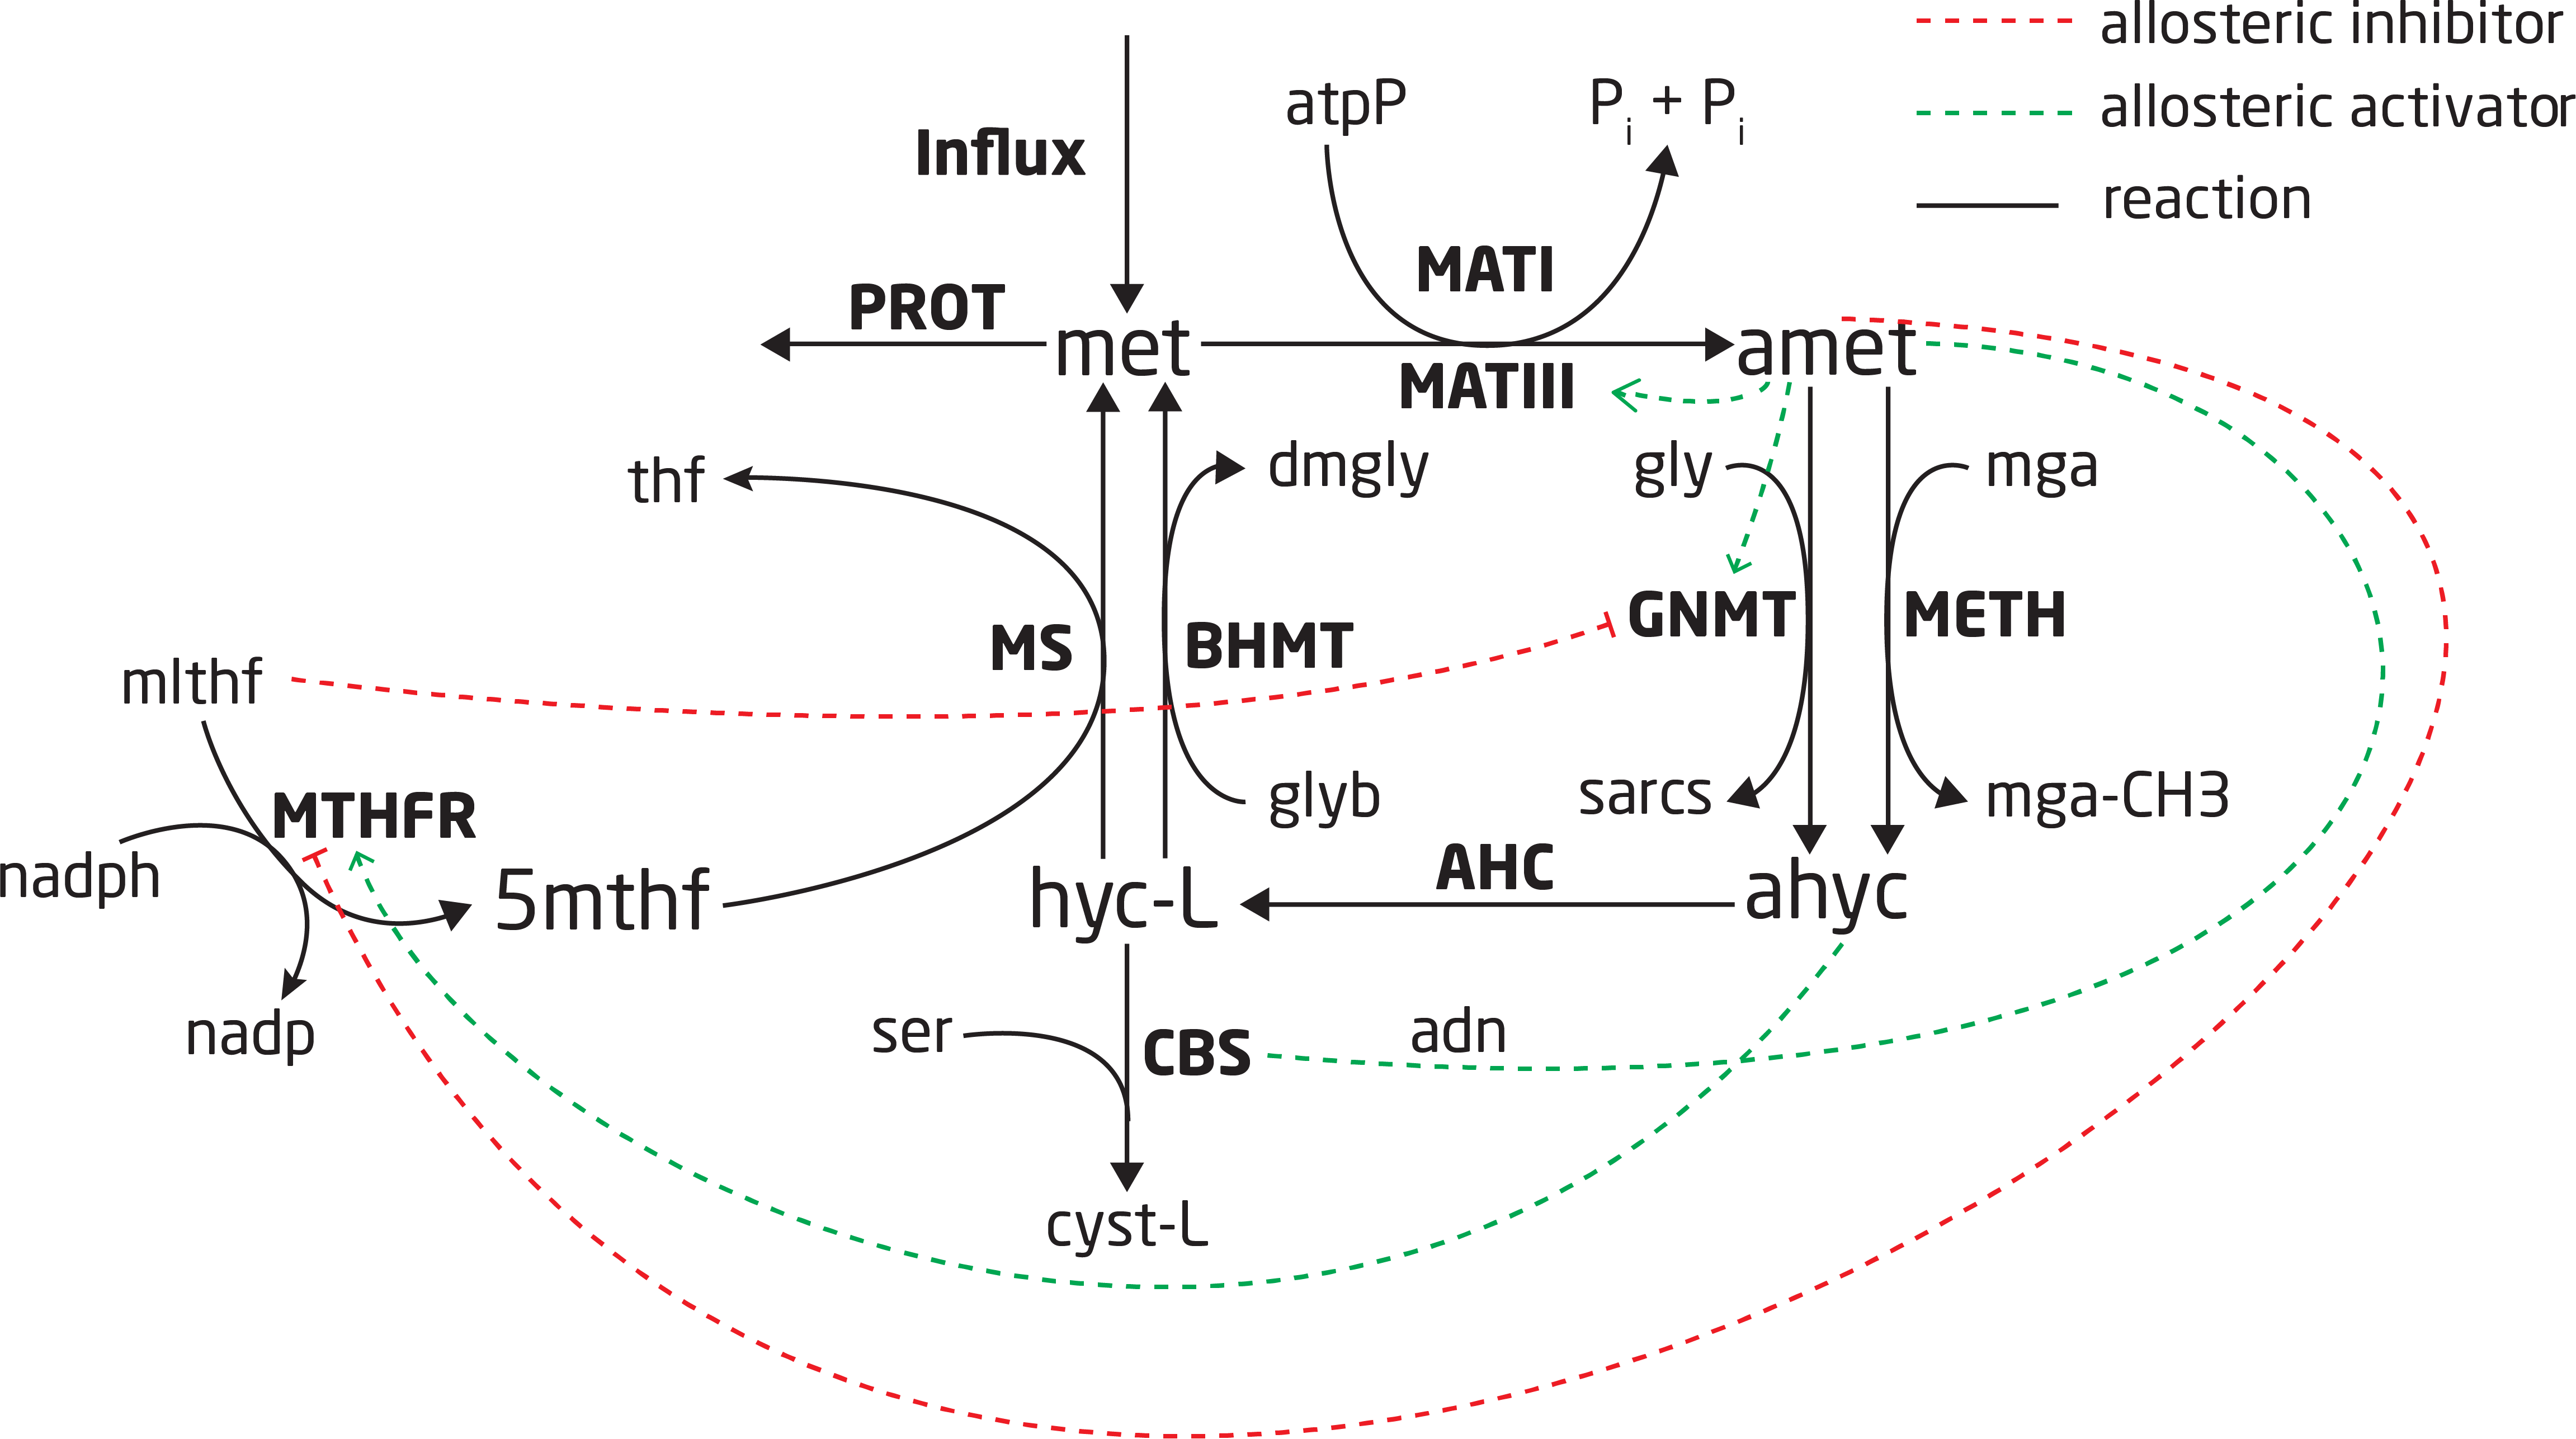
\includegraphics{../figures/methionine-reactions.png}

}

}

\end{minipage}%

\caption{\label{fig-methionine-reactions}The methionine cycle as
modelled, with the solid black lines representing the reactions, the
green lines representing allosteric interaction, and the red lines
representing allosteric inhibition. The bold fonts are the reaction
names and the regular font represents the metabolites.}

\end{figure}

\hypertarget{dataset-and-model-specification}{%
\subsection{Dataset and model
specification}\label{dataset-and-model-specification}}

The simulated dataset and underlying kinetic model that we used for our
analysis can be found at
\url{https://github.com/biosustain/Methionine_model/tree/main/data/methionine}
and is described in supporting information section 3.

We constructed a kinetic model of the methionine cycle in Maud's format
using the description in \citet{korendyaseva_allosteric_2008}. The
ordinary differential equation system describing this model is shown in
Equation\,\eqref{eq-meth-ode}.

\begin{align}
\frac{d[met]}{dt} &= v_{Influx} - v_{PROT} - v_{MAT} +v_{MS} + v_{BHMT} \label{eq-meth-ode} \\
\frac{d[amet]}{dt} &= v_{MAT} - v_{GNMT} - v_{METH} \nonumber \\
\frac{d[ahyc]}{dt} &= v_{GNMT} + v_{METH} - v_{AHC} \nonumber \\
\frac{d[hyc-L]}{dt} &= v_{AHC} - v_{CBS} - v_{MS} - v_{BHMT} \nonumber \\
\frac{d[5mthf]}{dt} &= v_{MTHFR} - v_{MS} \nonumber 
\end{align}

After specifying the qualitative aspects of the kinetic model, we
selected parameter values to use as ground truth by Monte Carlo sampling
using a previous model of the methionine cycle as a starting point (see
\citet{saa_construction_2016} for this model).

We used these parameters to simulate steady states in a range of
plausible experimental conditions, again using
\citet{saa_construction_2016} as a starting point. These steady states
were then used to generate simulated measurements using the measurement
model described below in Section~\ref{sec-methionine-measurement-model}.

\hypertarget{sec-methionine-measurement-model}{%
\subsubsection{Measurement
model}\label{sec-methionine-measurement-model}}

Generating an artificial dataset required a specification of the true
measurement error. For enzyme and metabolite concentration measurements
we specified a standard deviation of 0.1 on natural logarithmic scale,
corresponding to approximately 10\% measurement error. For each reaction
measurement a measurement standard deviation of approximately 10\% of
the simulated value.

These measurement error specifications are somewhat optimistic
considering the many sources of variation and uncertainty affecting
quantitative proteomics, metabolomics and fluxomics analyses, but are a
reasonable first approximation to a realistic set of measurements.

For our main model run, we assumed that all metabolite and enzyme
concentrations were measured, and that there was a reaction measurement
for each of the network's elementary flux modes.

\hypertarget{trainingvalidation-split}{%
\subsubsection{Training/validation
split}\label{trainingvalidation-split}}

The training testing split was selected to achieve a large difference
between the fluxes of the training and testing dataset. The split was
determined as we are interested in showing how our model can fit to
varied conditions, and conditions closer to the training set are likely
to be predicted well without necessarily learning the system.

\hypertarget{additional-dataset-with-missing-measurements}{%
\subsubsection{Additional dataset with missing
measurements}\label{additional-dataset-with-missing-measurements}}

To gain insight into our model's robustness to missing measurements, we
also performed a model run with the same 6 experimental datasets, but
with measurements of the metabolite S-Adenosyl-L-homocysteine, or
``ahcys'' removed. Since ahcys regulates three enzymes in the methionine
cycle, including one enzyme which is also thermodynamically regulated,
we expected the removal of these measurements to yield interesting
results.

\hypertarget{maud-input-specification}{%
\subsubsection{Maud input
specification}\label{maud-input-specification}}

We constructed inputs in Maud's format for each of the analysed
datasets, based on the scenario that the true kinetic model was known
except for parameter values, which needed to be inferred from the
training data and priors. These inputs can be found at
\url{https://github.com/biosustain/Methionine_model/tree/main/data}.

The prior distributions and corresponding true parameter values used in
our case study are shown in supporting information section 3.2. They
were chosen to reflect a plausible pre-experimental information state.
In 7 cases, the marginal prior distribution for a parameter disagrees
with the true parameter values used to generate the data. A similar
situation is likely to occur in practice due to \emph{in vivo} vs
\emph{in vitro} measurement differences.

\hypertarget{findings}{%
\subsection{Findings}\label{findings}}

\hypertarget{posterior-inference}{%
\subsubsection{Posterior inference}\label{posterior-inference}}

Running standard diagnostic checks indicated that the samples we
generated were from the target posterior distribution. The improved
\(\hat{R}\) statistic
\citep{vehtariRankNormalizationFoldingLocalization2021} for every
variable of interest was within 2\% of 1, indicating appropriate mixing
within and between Markov chains. Additionally, the number of effective
samples was high, indicating that we generated enough posterior samples
to support inferences about the bulks of the distributions of the
sampled parameters. Furthermore, we observed no post warm-up divergent
transitions, indicating that the sampler was able to transform the
log-posterior distribution, avoiding any regions with excessive
curvature that might inhibit exploration via HMC.

Posterior predictive checking indicated that our model achieved a good
fit to the simulated reaction and metabolite concentration measurements,
as shown by the graphs in the top row of figure
Figure~\ref{fig-posterior}.

Analysis of the posterior distributions for kinetic parameters indicated
that these are highly correlated. The marginal posterior distributions
for most kinetic parameters did not shrink significantly compared with
the corresponding marginal prior distributions, even though these
parameters' joint posterior distribution contained enough information to
make accurate out of sample predictions. In some cases, there were
two-dimensional correlations such as the one shown in the bottom left of
figure Figure~\ref{fig-posterior}; in this case the marginal
distribution of the two parameters is roughly banana shaped. More
commonly, however, two-dimensional pair plots were insufficient to
reveal the underlying correlation structure, as seen in the bottom-right
plot in figure Figure~\ref{fig-posterior}. This does not mean that the
parameters were uncorrelated, but rather that the correlations involve
more than two parameters.

Overall, our results show that Maud can fit a realistic pathway-sized
dataset. This was achieved without fixing the marginal values of kinetic
parameters: the information required to make good predictions was
contained in the correlation structure of the joint posterior
distribution. This finding is consistent with previous analyses of
biological systems that found they are ``sloppy'', that is, sensitive to
parameter combinations rather than marginal parameter values, with
important combinations, scales and regions of sensitivity being
difficult to ascertain in advance
\citep{gutenkunst_2007, poirier_revising_1998}.

The question naturally arises whether the crucial high-dimensional
parameter correlations are linear or non-linear. This is relevant to the
question of model performance, as linear correlations are easier to
correct for. A linearly correlated posterior space would also be easier
to summarise. We address this question below in
Section~\ref{sec-laplace}.

This case study illustrates the type of kinetic model and dataset that
Maud can fit. The model we analysed has 10 reactions, 5 state variables
and 212 parameters. Generalising from our ability to fit this model in a
reasonable time using Maud, we expect that Maud can be used to fit
realistic Bayesian models of approximately the same size, but not, for
example, genome-scale kinetic models. To fit larger models, faster
steady state solving methods or alternative inference algorithms will be
required. Section~\ref{sec-laplace} addresses whether Laplace
approximation is a suitable candidate.

\begin{figure}

\begin{minipage}[t]{\linewidth}

{\centering 

\raisebox{-\height}{

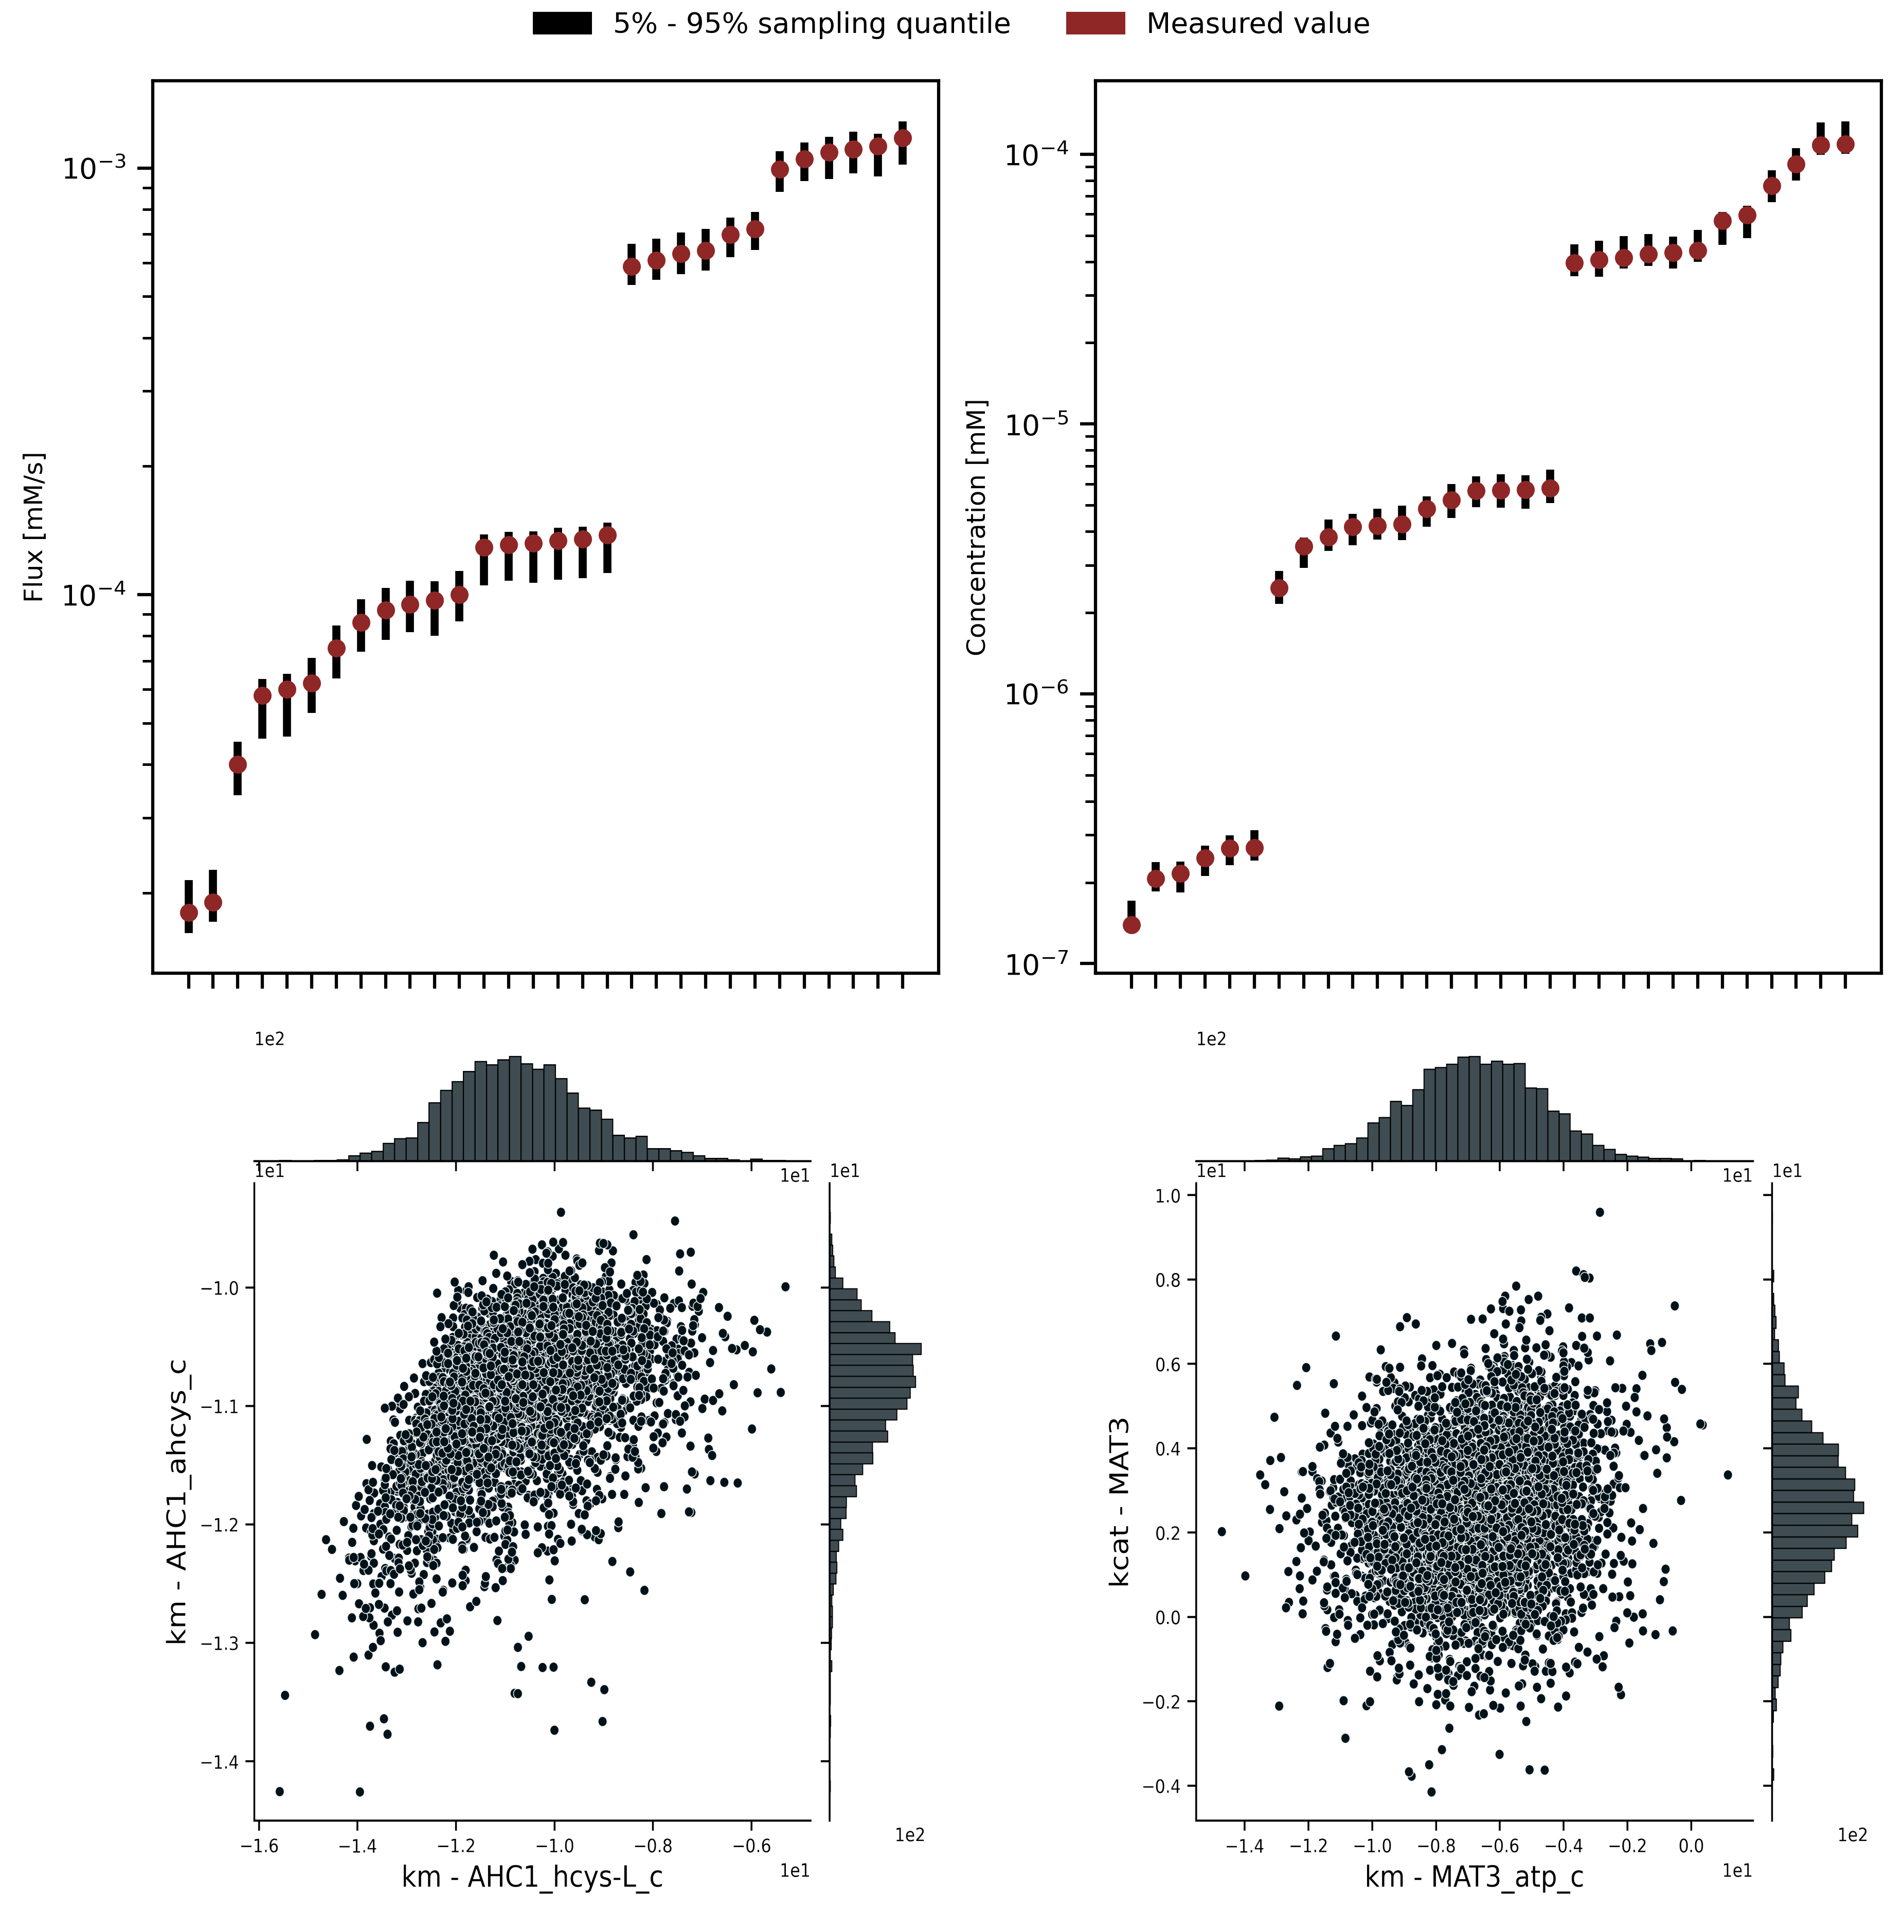
\includegraphics{../figures/posterior.png}

}

}

\end{minipage}%

\caption{\label{fig-posterior}Marginal posterior distributions from our
main model run. (\textbf{Top left}) Comparison of posterior predictive
intervals with simulated flux measurement values. All the flux
measurements are within the predictive intervals, indicating a good fit.
(\textbf{Top right}) Comparison of posterior predictive intervals with
simulated concentration measurement values. These also show a good fit.
(\textbf{Bottom left}) Pairwise marginal posterior distribution for two
uncorrelated parameters, namely \(K_m^{AHC1,hcys-L}\) and
\(K_m^{AHC1_ahcys}\). (\textbf{Bottom right}) Pairwise marginal
posterior distribution for two correlated parameters, namely
\(K_m^{MAT3,atp}\) and \(K_{cat}^{MAT3}\).}

\end{figure}

\hypertarget{sec-laplace}{%
\subsubsection{Comparison with Laplace
approximation}\label{sec-laplace}}

We found that the Laplace method was not able to produce an accurate
posterior approximation for our model and dataset.

Our overall strategy was to compare samples generated using MCMC, which
we were confident could be treated as draws from the true posterior
distribution, with approximate posterior samples generated using the
Laplace method. We were unable to generate approximate posterior samples
for our main methionine cycle case study using Laplace approximation, as
the algorithm could not recover from solver failures caused by
unrealistic parameter configurations. We therefore made a comparison for
a simpler model. This input can be found at
\url{https://github.com/biosustain/Methionine_model/tree/main/data/example_ode}.

MCMC sampling for our comparison input yielded 800 samples in 625
minutes; Laplace sampling yielded the same number of samples in only one
minute. The diagnostics indicated that our algorithm was able to find
the maximum a posteriori parameter configuration, approximate the
Hessian and use these quantities to generate approximate posterior
samples. The results can be found at
\url{https://github.com/biosustain/Methionine_model/tree/main/results}.

Figure~\ref{fig-laplace} summarises the results of comparing the samples
generated using each method. As can be seen from the top left plot, the
Laplace method does not provide a good approximation to the true
posterior distribution in this case, as the marginal distribution of the
total log probability density is clearly different. This impression was
confirmed using the Kolmogorov-Smirnov test, which is a test to
differentiate two empirical univariate distributions. The two
distributions were significantly different with a p-value
indistinguishable from zero.

The difference between the Laplace approximation output and the true
posterior distribution manifests not only in the parameter space, but
also in the measurement space. Figure Figure~\ref{fig-laplace} frame B
compares the 5\%-95\% interval for flux measurement log likelihoods in
the true posterior with the Laplace approximation; lower log likelihood
values indicate that the modelled and measured values are further away.
The graph shows that the Laplace approximation yielded significantly
worse predictions than the true posterior, even for the training data.

To further explore why this is the case we compared samples from the
true posterior and the Laplace approximation for the pairwise marginal
distributions of two Michaelis-Menten constants \(K_{m}^{A,r1}\) and
\(K_{cat}^{r1}\): see the bottom right cell of figure
Figure~\ref{fig-laplace}. This comparison demonstrates that the Laplace
method is not able to capture the correct relationships between
parameters' distributions.

This result shows that MCMC, while slower than Laplace approximation, is
unfortunately preferable for posterior inference in this case. We expect
that the Laplace method will produce worse approximations the more
complex the target model. Since the approximation is already
unacceptable for our simple test model, we recommend that Maud users use
MCMC sampling in preference to Laplace approximation if possible when
fitting realistic Bayesian kinetic models.

Our results here also provide circumstantial evidence that the parameter
correlations in Bayesian kinetic model posteriors tend to be non-linear,
as a posterior with only linear correlations would likely be more
germane to Laplace approximation. A conclusion that we drew from this
analysis was that the results of fitting our model cannot be summarised
simply, for example by fitting a multivariate normal distribution to the
posterior draws. We therefore recommend that Maud users store the full
set of MCMC draws rather than using such an approximation. This does not
preclude the possibility that there is an alternative, more compact, way
to summarise the results of Bayesian kinetic model inference; we leave
research into this topic to future work.

\begin{figure}

\begin{minipage}[t]{\linewidth}

{\centering 

\raisebox{-\height}{

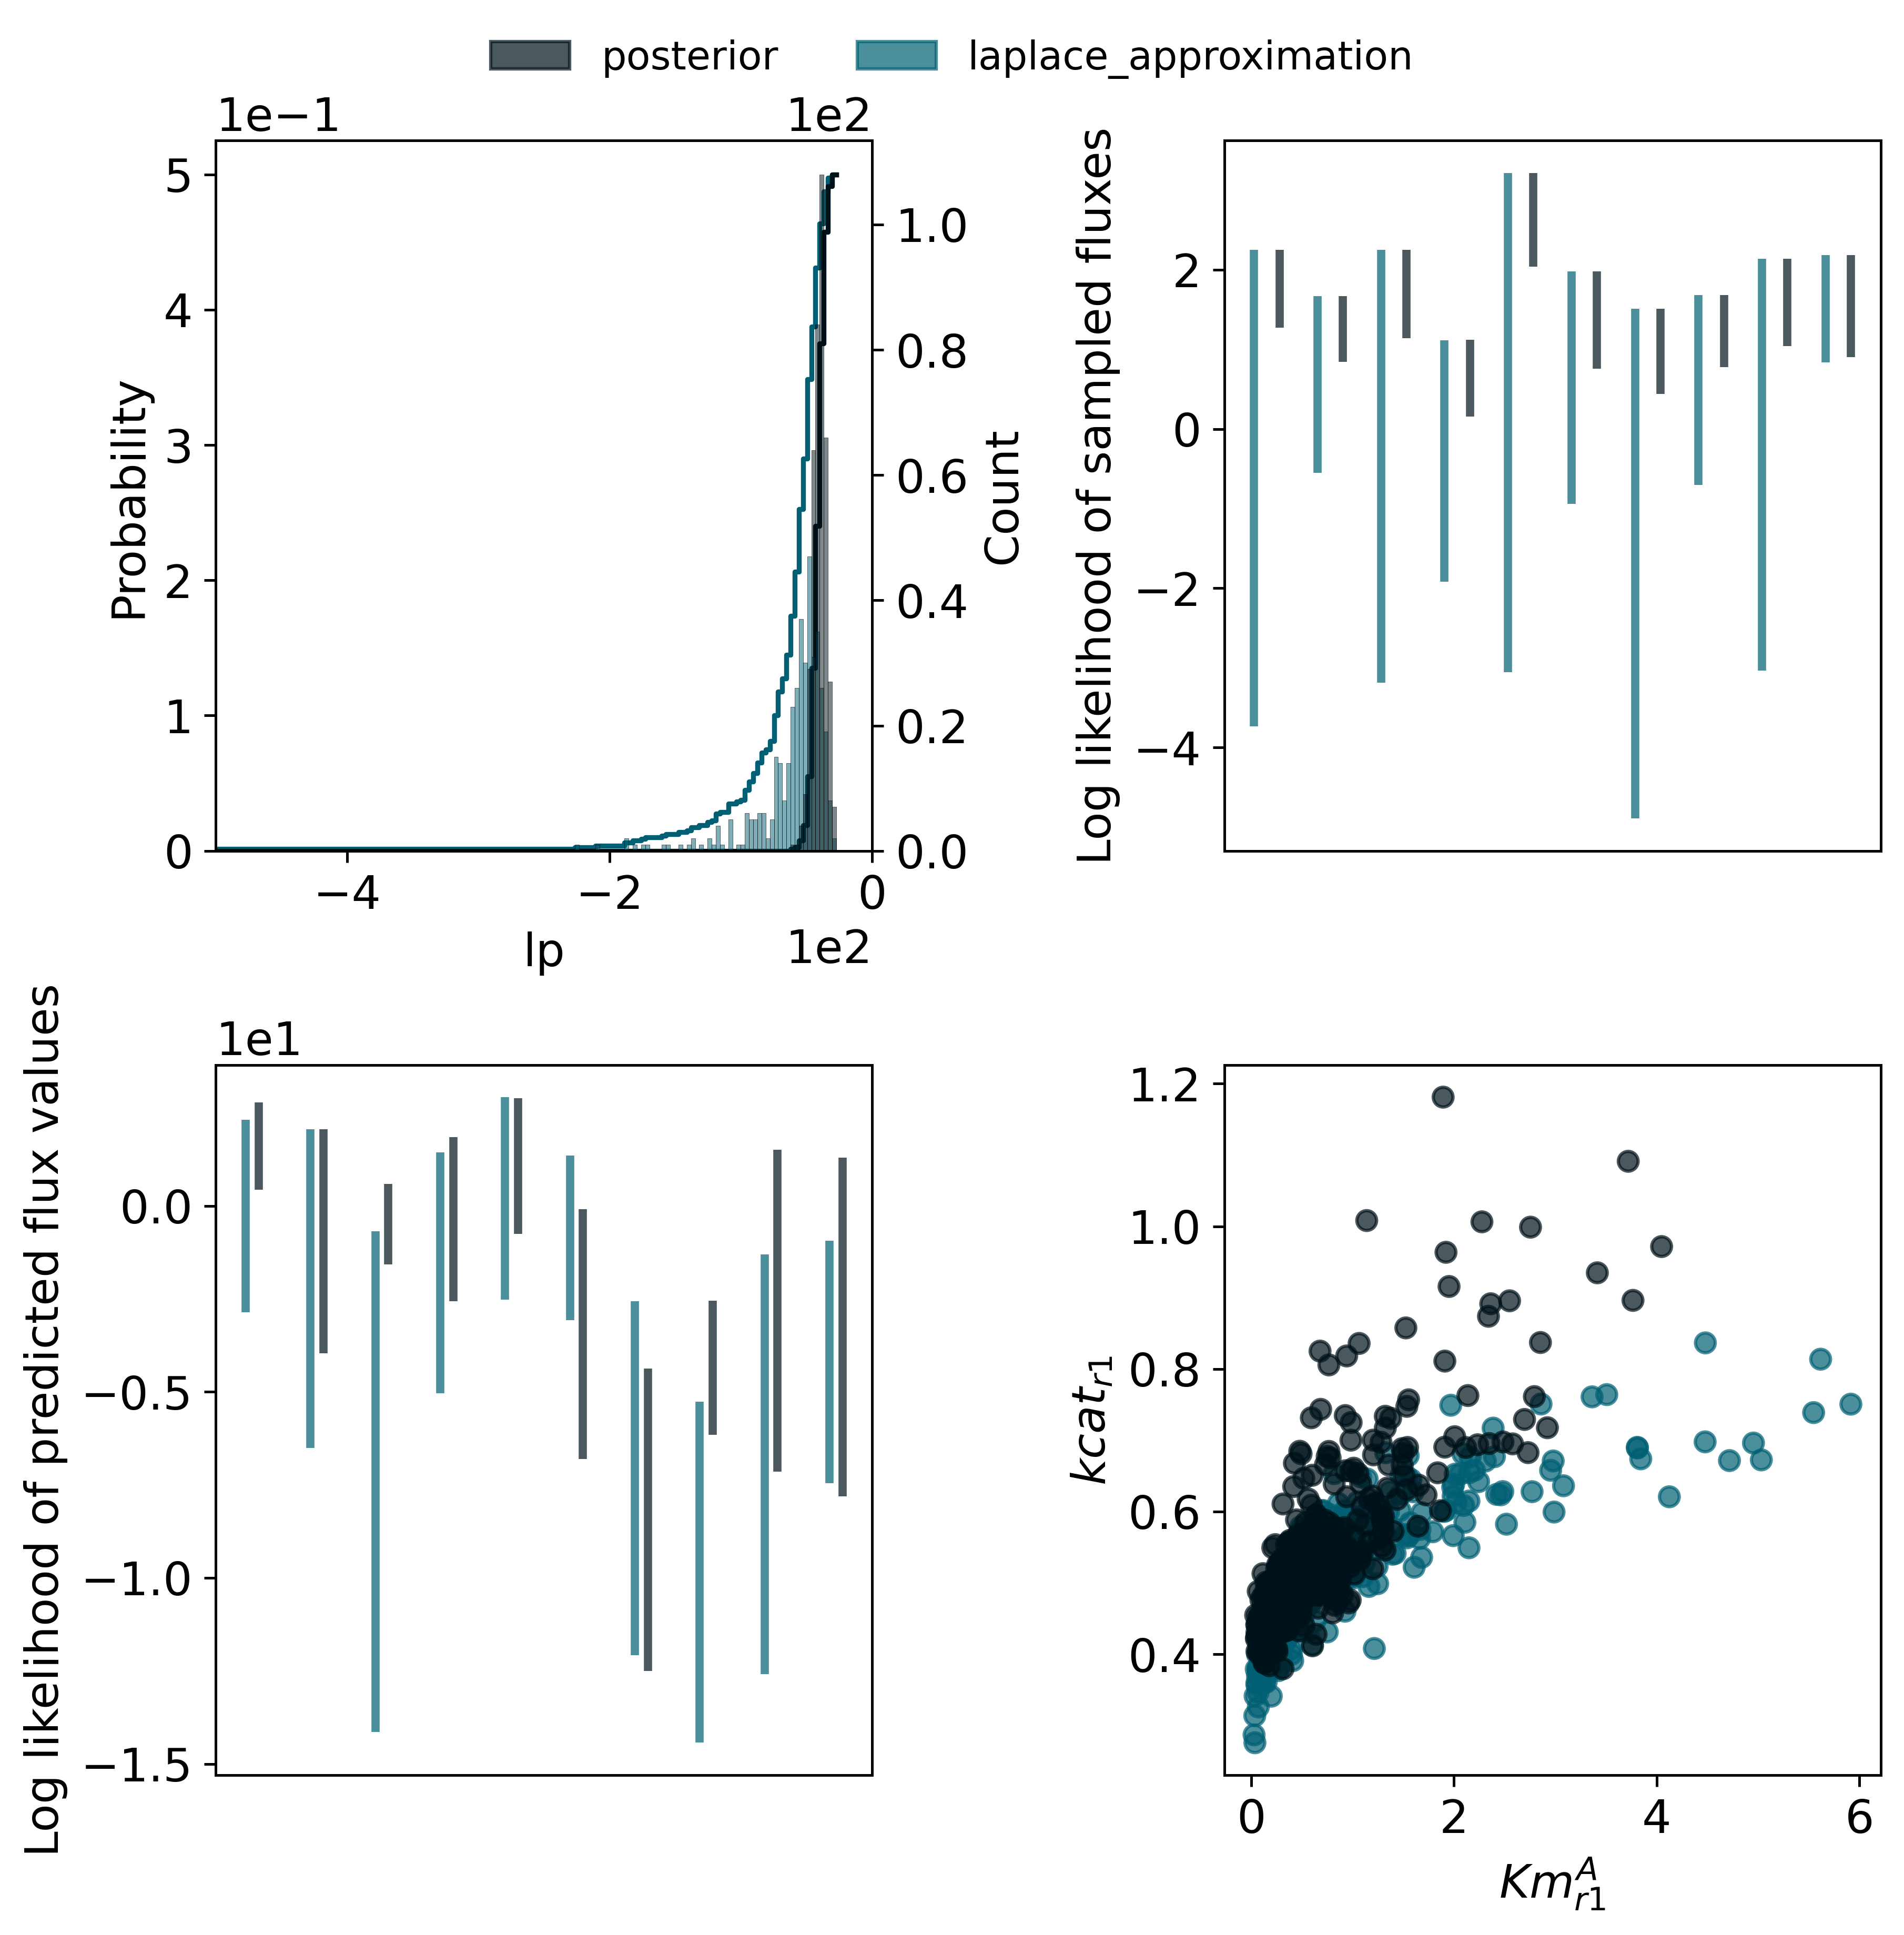
\includegraphics{../figures/laplace.png}

}

}

\end{minipage}%

\caption{\label{fig-laplace}Graphical comparison of approximate
posterior samples generated using Laplace sampling (blue-green) with
posterior samples generated using MCMC (dark grey). (\textbf{Top left})
the two sets of samples clearly have different marginal distributions
for the overall log probability variable, indicating that the Laplace
samples do not accurately approximate the target distribution.
(\textbf{Top right}) The distribution of marginal posterior predictive
log likelihood values for training data flux measurements shows that the
Laplace method tended to yield much worse predictions compared with the
true model. (\textbf{Bottom left}) The Laplace method also tended to
produce worse flux predictions for held-back test measurements.
(\textbf{Bottom right}) The marginal joint distribution of two
parameters: \(K_m^{A,rl}\) and \(K_{cat}^{r1}\). The Laplace method is
not able to track the correct joint distribution for this pair of
parameters. This is unsurprising given that the target distribution has
position-dependent scales which are difficult for a linear approximation
to capture.}

\end{figure}

\hypertarget{effect-of-missing-metabolite-concentration-measurements}{%
\subsubsection{Effect of missing metabolite concentration
measurements}\label{effect-of-missing-metabolite-concentration-measurements}}

Comparing model runs with and without the ahcys measurements showed that
Maud can produce sensible results even from incomplete metabolomics
data.

Figure~\ref{fig-missing} shows that, as might be expected, the model
with missing measurements did not correctly infer the missing ahcys
concentrations. Nonetheless, the remaining measured metabolites were
still well predicted, suggesting that information about the network is
still preserved despite the missing measurements. Comparison of flux
measurements in both models also indicated that removing the ahcys
measurement did not result in catastrophic model failure.

The missing measurements did affect Maud's ability to infer parameter
values correctly. The lower left plot of Figure~\ref{fig-missing} shows
that the model with full metabolomics learned the true value for the
displayed dissociation constant, despite this value being far from the
mean of the corresponding marginal prior distribution. In contrast, the
model with missing measurements stayed in the neighbourhood of the
prior.

This result is reassuring because not having access to all measurements
is a common situation in multi-omics studies. For instance, measuring
all metabolites in a pathway can be infeasible because of limitations of
mass spectrometers, availability of standards, column effects, and
compartmentalisation. However, provided that sufficient information is
available from other sources, our approach can produce sensible results
from incomplete metabolomics data.

\begin{figure}

\begin{minipage}[t]{\linewidth}

{\centering 

\raisebox{-\height}{

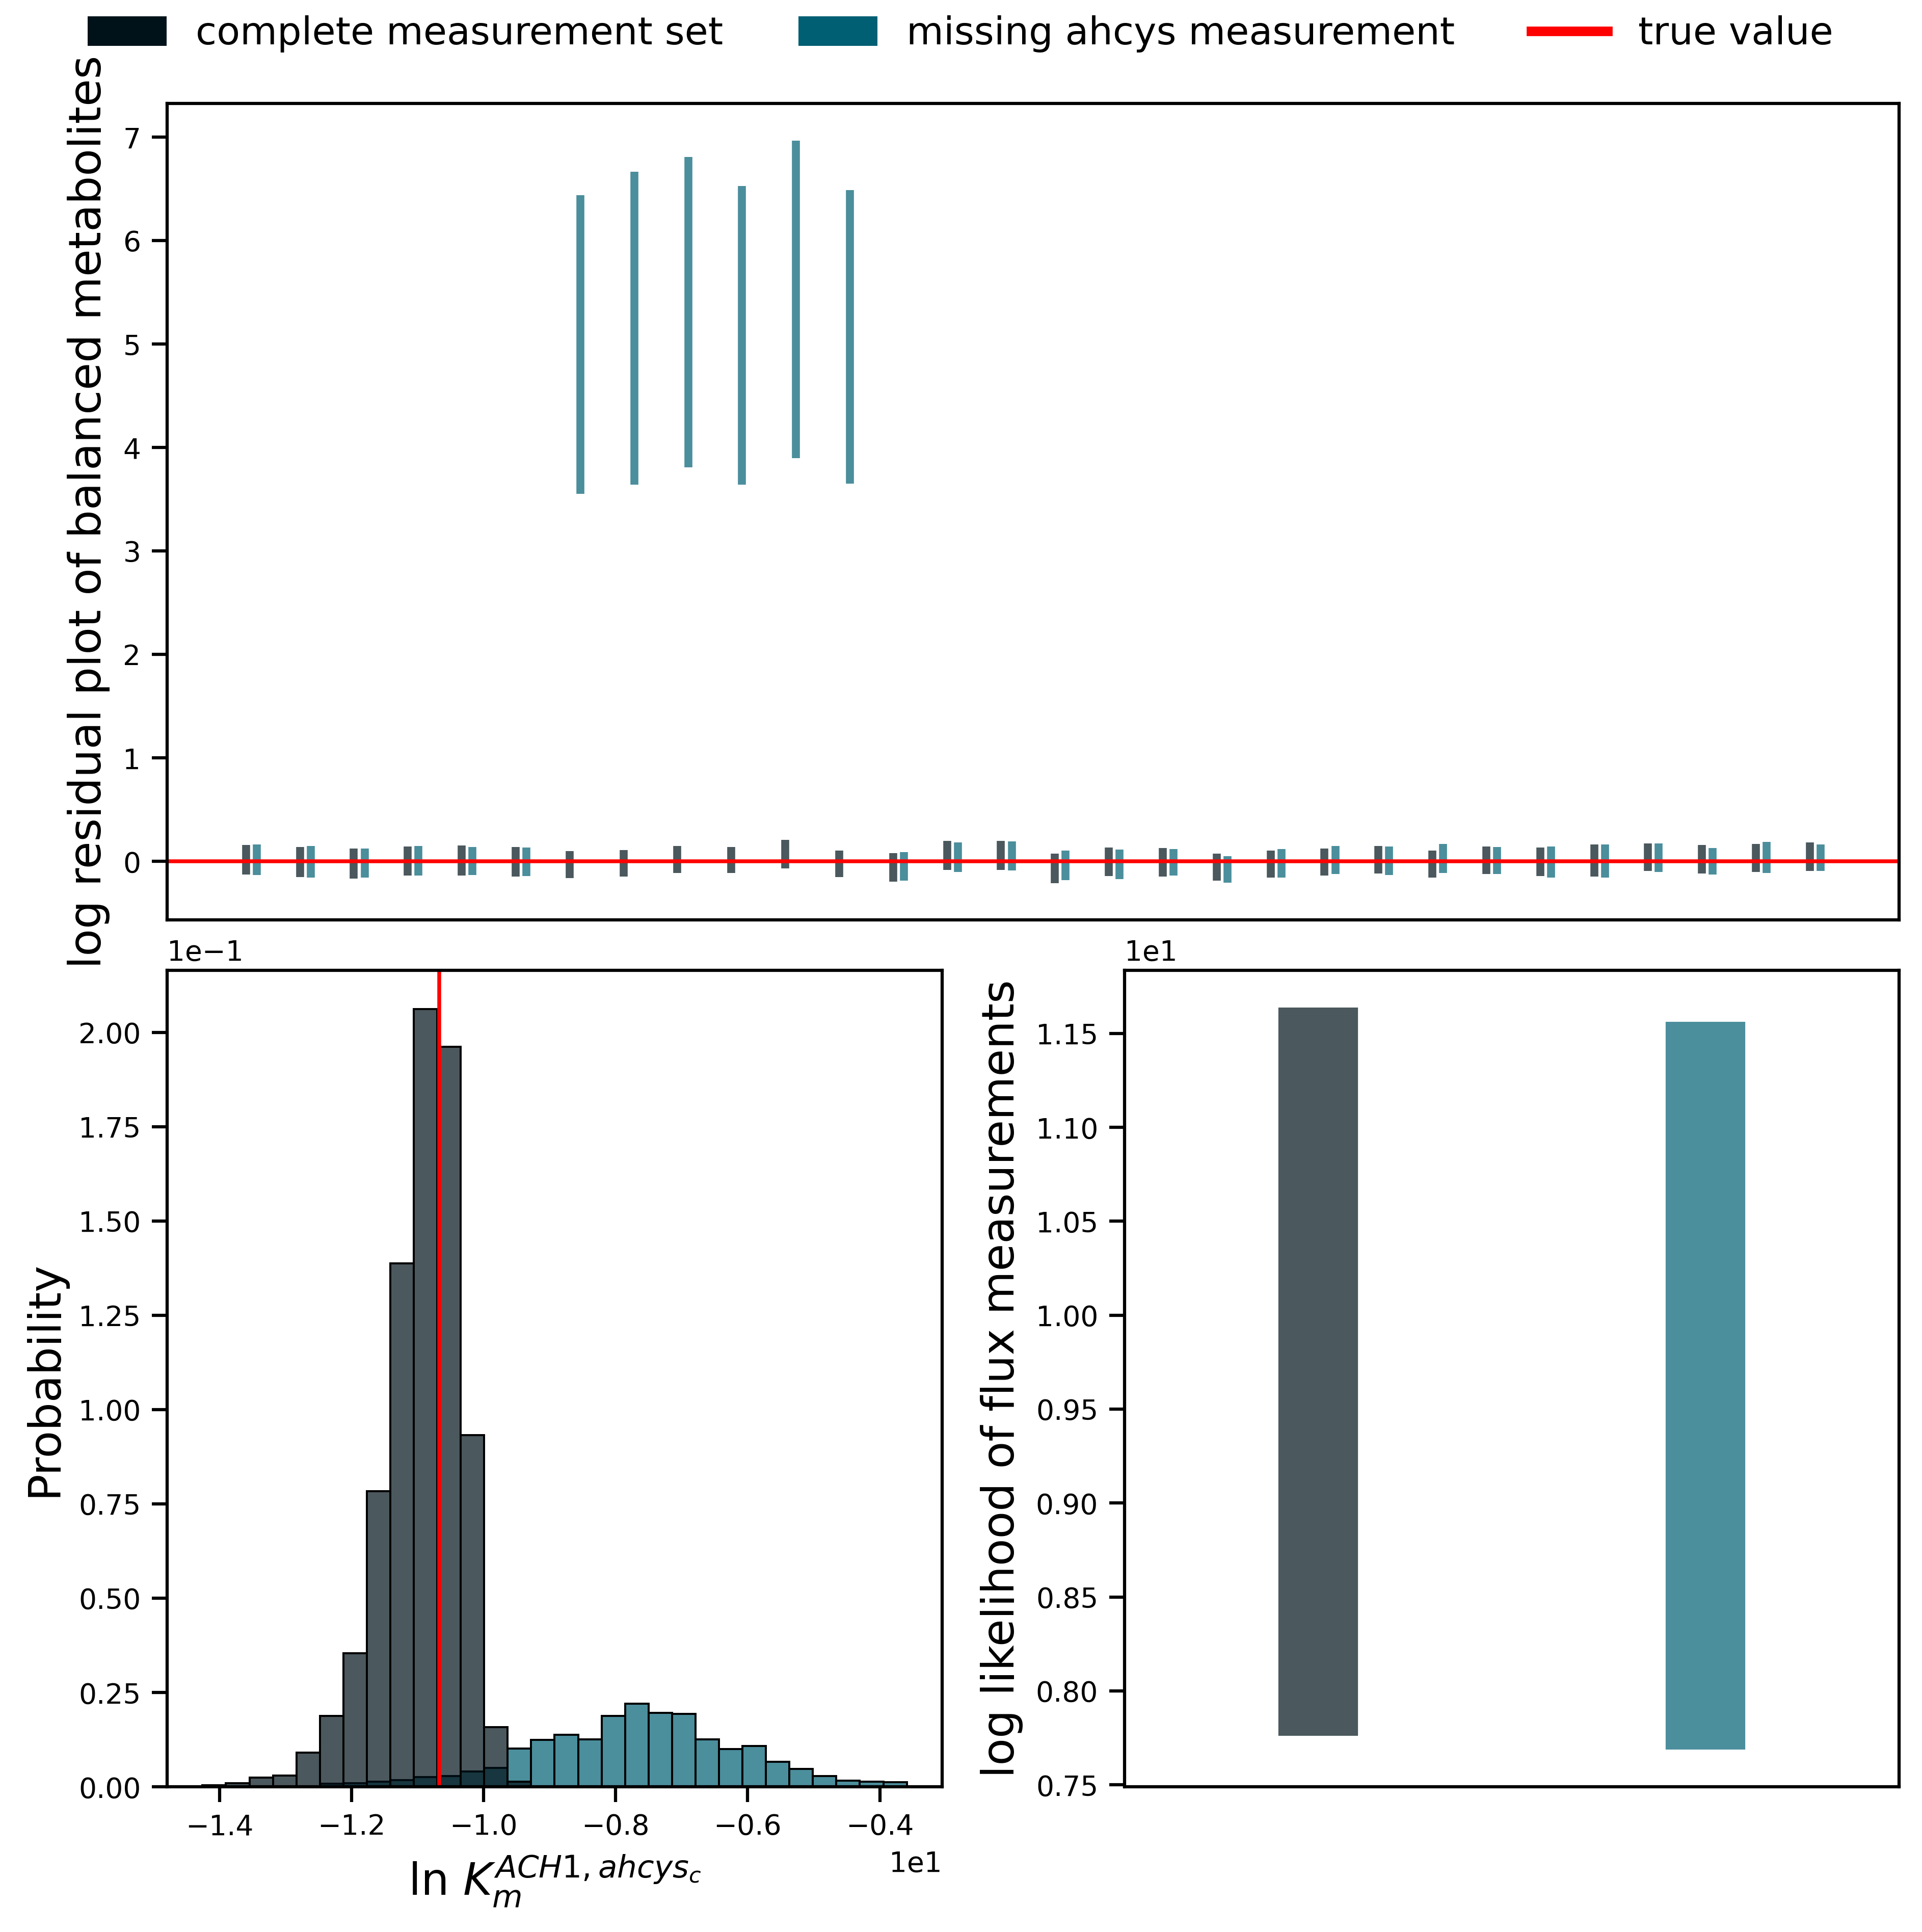
\includegraphics{../figures/missing.png}

}

}

\end{minipage}%

\caption{\label{fig-missing}Results of removing concentration
measurements for the metabolite \(ahcys_c\) from our case study dataset.
(\textbf{Top}) A comparison of metabolite concentration residuals
between the full measurement dataset (blue-green) and the missing-data
dataset (grey), displayed on natural logarithmic scale. The missing-data
model was unable to estimate the withheld \(ahcys_c\) concentrations.
(\textbf{Bottom Left}) The marginal posterior distribution for the
Michaelis constant \(K_m^{AHC1,ahcys_c}\) in each model, alongside the
true parameter value used to generate both datasets. The true value is
recovered by the complete-data model but not by the missing-data model.
(\textbf{Bottom Right}) The distribution of total log-likelihood for
out-of-sample flux measurements in both models. There is a significant
overlap between the two distributions, suggesting that removing the
\(ahcys_c\) measurement did not cause catastrophic prediction failure.
However, overall the complete-data model tended to make better
predictions.}

\end{figure}

\hypertarget{application-to-regulatory-understanding}{%
\subsubsection{Application to regulatory
understanding}\label{application-to-regulatory-understanding}}

To demonstrate how Maud's output can be used to yield useful metabolic
insights we used the results of our case study to explain why the flux
of the enzyme \(GNMT\) is higher in dataset 1 than in dataset 12. GNMT
is an irreversible enzyme that is homotropically activated by its
substrate, competitively inhibited by its product and heterotropically
inhibited by 5,10- methylenetetrahydrofolate (mlthf). The diverse
regulation makes it the ideal test case to elucidate regulatory changes.

Figure~\ref{fig-decomposition} shows the regulatory description of GNMT,
according to the results our main case study analysis. Each curve shows
the marginal posterior distribution of the ratio of the corresponding
regulatory component in dataset 1 compared with dataset 12. A positive
value indicates that the component was increased in dataset 1 relative
to dataset 12, with 0 indicating no difference. The probability,
according to our model, of the component acting in each direction is
given by the relative area under the curve on each side of the 0 point.

Our model correctly inferred that saturation and allosteric effects were
the main drivers of regulation between the two datasets in this case,
with the curves for each component aligning with the ground truth shown
in red.

Importantly, this form of analysis takes into account all modelled
sources of uncertainty, including uncertainty about the measured values
of the flux in each dataset. Our result shows that Maud could be used in
this realistic case not only to provide a user with an explanation for
an observed difference in fluxes, but also a reasonable judgement as to
the explanation's robustness.

\begin{figure}

\begin{minipage}[t]{\linewidth}

{\centering 

\raisebox{-\height}{

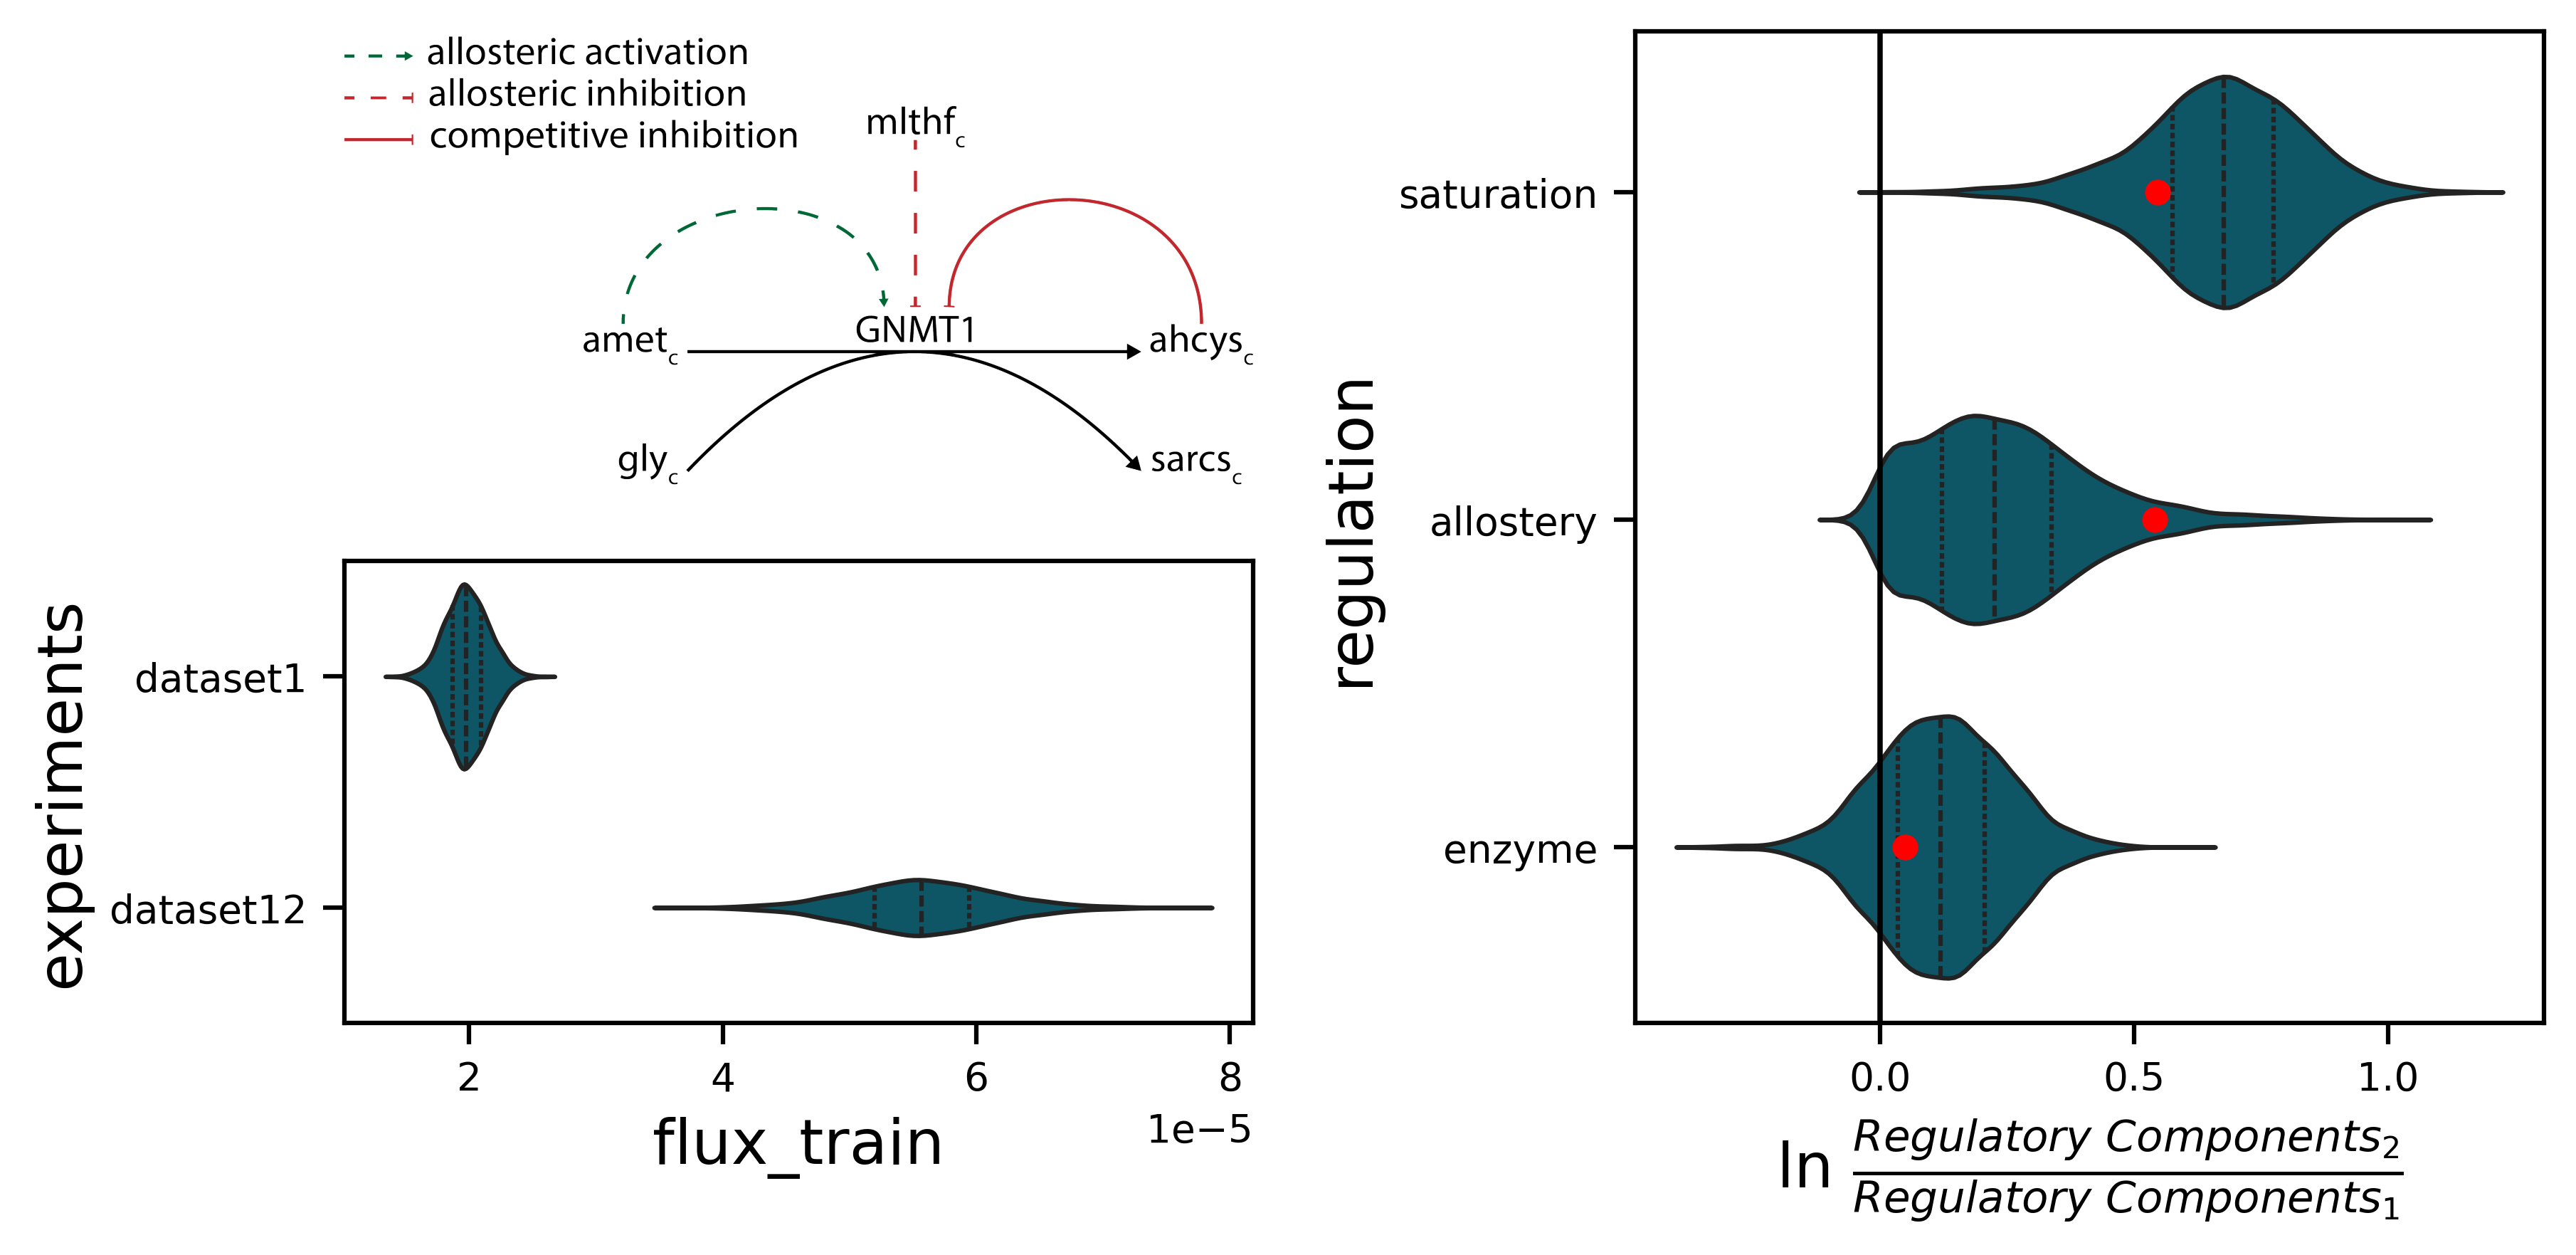
\includegraphics{../figures/decomposition.png}

}

}

\end{minipage}%

\caption{\label{fig-decomposition}Illustration of how analysing a system
with Maud can yield actionable insights about the underlying metabolic
network. (\textbf{Top Left}) A schematic of the regulatory interactions
associated with the enzyme \(GNMT1\). Dashed green lines represents
allosteric activation, dashed red lines indicate allosteric inhibition
and solid red lines represent competitive inhibition. (\textbf{Bottom
Left}) Comparison of marginal posterior distributions for \(GNMT\) flux
in datasets 1 and 2. (\textbf{Right}) Log-scale ratios of the regulatory
elements defined in equation \eqref{eq-decomposition}. Note that the
\(Reversibility\) and \(k_cat\) components are excluded: this is because
this reaction was modelled as irreversible, and \(k_{cat}\) was modelled
as constant across datasets. These plots identify why flux in dataset 12
is higher than in dataset 1: the flux increase is due to allostery and
saturation with no control from enzyme concentration changes.}

\end{figure}

\hypertarget{methods}{%
\section{Methods}\label{methods}}

Maud is a command line application implementing Bayesian inference for a
wide range of realistic kinetic models. Maud is written in Python
\citep{vanrossumPythonReferenceManual2009}, designed for use on Windows,
macOS and Linux, is \texttt{pip} installable from the Python Package
Index as \texttt{maud-metabolic-models}, documented at
\url{https://maud-metabolic-models.readthedocs.io} and actively
developed and maintained at \url{https://github.com/biosustain/Maud/}.

To use Maud, a user must first collate appropriate input information,
represent it in files with Maud's required formats (see supporting
information section on input format). Maud's command line interface
provides commands for inference via a range of algorithms including
adaptive Hamiltonian Monte Carlo, as well as commands for simulation and
making out-of-sample predictions. Results are stored in files, using a
structured, interoperable format.

As well as parameter values, Maud also performs inference for derived
quantities including the components of the regulatory decomposition
described below in equation \eqref{eq-decomposition}, log likelihoods,
simulated measurement values and metabolic control analysis coefficients
\citep{kacser_control_1973}.

In the rest of this section we describe Maud's kinetic model at high
level and discuss Maud's statistical model, implementation and how it
solves the crucial steady state problem. Further details about Maud's
kinetic model can be found in the supporting information.

\hypertarget{kinetic-model}{%
\subsection{Kinetic model}\label{kinetic-model}}

Maud's kinetic model decomposes into factors as shown in equation
\eqref{eq-decomposition}.

\begin{equation}
F(C;\theta) = Enzyme\cdot k_{cat}\cdot Reversibility \cdot Saturation \cdot Allostery \label{eq-decomposition}
\end{equation}

Each of the terms on the right-hand side of \eqref{eq-decomposition} is
a function of \(C\) and \(\theta\). This idea is taken from
\citet{noor_note_2013}. The terms usefully gather physically meaningful
and conceptually distinct factors contributing to reaction fluxes.
\(Enzyme\) captures the effect of enzyme concentration, \(k_{cat}\) that
of enzyme efficiency, \(Reversibility\) quantifies thermodynamic
effects, \(Saturation\) the effect of enzyme availability and
\(Allostery\) the effect of post translational modifications.

We used the model of enzyme saturation from
\citet{liebermeister_modular_2010} and the generalised
Monod-Wyman-Changeux model of Allosteric regulation introduced in
\citep{monod_nature_1965, changeux_2013, popova_generalization_1975, popova_description_1979}
and used more recently in \citet{matosGRASPComputationalPlatform2022}.
To capture the effect on enzyme activity of coupled phosphorylation and
dephosphorylation processes we developed a new mathematical model
inspired by the generalised MWC model of allosteric regulation. Full
details of all mathematical aspects of Maud's kinetic model can be found
in supporting information section 2.

\hypertarget{statistical-model}{%
\subsection{Statistical model}\label{statistical-model}}

Maud represents information from measurements using generalised linear
regression models that probabilistically connect realised measurements
with true values of the measurable quantities. Information from other
sources is represented using a prior distribution over a set of latent
parameters. The parameters and the measurable quantities are connected
by a generative model encompassing Maud's kinetic model as well as the
steady state equation \eqref{eq-3}. Together, the measurement model,
prior model and generative model determine a joint probability function
that assigns a probability density to any possible combination of
measurements and parameters.

Below we describe the prior and measurement models, as the generative
model has already been discussed above.

\hypertarget{prior-model}{%
\subsubsection{Prior model}\label{prior-model}}

Maud's prior model includes unknown parameters corresponding to
quantities in the kinetic model that are assumed to be unknown, other
than steady state metabolite concentrations and fluxes, which are
derived from the values of other parameters by solving the steady state
problem. See table (REFERENCE) in this paper's supporting information
for a description of all these parameters and their dimensions. Note
that some quantities in Maud's kinetic model are not treated as
parameters: for example, temperatures, compartment volumes and the
formation energy of water. Maud treats these quantities as if they were
known precisely: they can be configured by the user or default values
can be used. Although in practice there can be considerable uncertainty
regarding these quantities, we chose to disregard this uncertainty in
the interest of simplicity.

Except for metabolites' standard condition Gibbs energy changes of
formation, Maud uses independent normal prior distributions for
parameters that can in principle be both negative and positive. For
parameters that are constrained to be positive, Maud uses independent
log-normal distributions. Formation energy parameters have a
multivariate normal prior distribution. Location, scale and covariance
parameters for all these prior distributions can be selected freely by
the user.

\hypertarget{measurement-model}{%
\subsubsection{Measurement model}\label{measurement-model}}

Maud's measurement model considers three types of measurement:
metabolite concentration measurements, enzyme concentration measurements
and flux measurements, represented by vectors \(𝑦^{𝑐𝑜𝑛𝑐}\) \(𝑦^{𝑒𝑛𝑧}\)
and \(𝑦^{𝑓𝑙𝑢𝑥}\) respectively.

All measurements are specific to an experimental condition; that is, a
case where the true state of the network, including knockouts, boundary
conditions and state variables as well as kinetic and thermodynamic
parameters, can safely be assumed to be the same. Maud's statistical
model allows for arbitrarily many experimental conditions, and for any
measurable quantity to be measured any number of times in any condition.

Metabolite and enzyme measurements are intended to represent the results
of quantitative metabolomics and proteomics experiments. The likelihood
functions for such measurements are shown in equations
Equation\,\eqref{eq-yconc} and Equation\,\eqref{eq-yenz}.

\begin{align}
y_i^{conc} &\sim LN(\ln{\hat{y}_i^{conc}}, \sigma_i^{conc})\label{eq-yconc} \\
y_i^{enz} &\sim LN(\ln{\hat{y}_i^{enz}}, \sigma_i^{enz})\label{eq-yenz}
\end{align}

Both equations are log-normal generalised linear models with a standard
link function (the natural logarithm \(\ln\)) and known standard
deviation \(\sigma_{𝑐𝑜𝑛𝑐}\). The use of this measurement model is
motivated by the consideration that concentrations are constrained to be
non-negative, so the measurement model should avoid assigning positive
probability mass to negative metabolite concentration values. In
addition, we expect the precision of most metabolomics and proteomics
experiments to be roughly proportional to the value of the true measured
quantity, which supports a measurement model with constant coefficient
of variation. The measurement standard deviations \(\sigma_{𝑐𝑜𝑛𝑐}\) and
\(\sigma_{𝑒𝑛𝑧}\) are assumed to be known exactly for simplicity;
plausible values can be elicited by considering the likely coefficient
of variation of the measuring apparatus.

Flux measurements, representing the results of quantitative fluxomics
analyses, are modelled using a likelihood function from a standard
linear regression model, as shown in equation\,\eqref{eq-yflux}. Flux
measurements can be obtained from the results of isotope labelling
experiments using metabolic flux analysis, for example as described in
(Young 2014). When entering flux measurements, it is important only to
specify measurements for a network's free fluxes, as the values of some
steady state fluxes in a metabolic network are constrained by others,
with the result that dependent fluxes cannot typically be measured
separately. If measurements of multiple dependent fluxes are entered,
information will inappropriately be double counted.

\begin{equation}
y_i^{flux} \sim LN(\ln{\hat{y}_i^{flux}}, \sigma_i^{flux})\label{eq-yflux}
\end{equation}

Our measurement model improves on analyses of metabolomics and
proteomics data that assume a regression model with normally distributed
errors, whether explicitly using a standard linear model or implicitly
using ordinary least squares fitting. This assumption is undesirable
because it implies that the measured quantity could in principle be
negative, and assumes an additive underlying random process, whereas
multiplicative processes tend to better describe real concentration
data.

The use of independent measurement models for metabolite, enzyme and
flux measurements carries an implicit assumption that there are no
systematic correlations in the measurement errors. This choice was
motivated by simplicity - it would be better to use a model with
potentially correlated measurements. Similarly, it would be preferable
to include measurement errors as model parameters, thereby avoiding
possible bias due to incorrect assessments of measurement accuracy.
However, we chose to use a simpler measurement model to avoid the
complexity and potential fitting issues that these changes would entail.

Finally, the reader may wonder why Maud uses a linear regression model
for reaction flux measurements even though this creates the potential
for erroneous double counting and requires non-trivial upstream
modelling, as intracellular fluxes typically cannot be measured
directly. Instead, fluxes are typically inferred from isotope labelling
experiments using metabolic flux analysis: see
\citet{daiUnderstandingMetabolismFlux2017} for more about this method.
Ideally Maud's measurement model for fluxes would extend from fluxes to
the results of potential labelling experiments, thereby removing the
need for upstream analysis and avoiding any double counting. This option
has not yet been pursued, again for the sake of simplicity.

\hypertarget{implementation}{%
\subsection{Implementation}\label{implementation}}

Maud uses the Python library click
\citep{clickdevelopersClickPythonComposable2022} to implement a command
line interface. The command line interface loads input files as Python
dictionaries, which are parsed using the Python library \texttt{toml}
\citep{pearsonTomlPythonLibrary2020} and then validated and converted
into structured \texttt{MaudInput} objects using Pydantic
\citep{pydanticdevelopersPydantic2022}. Maud's statistical model is
implemented in the probabilistic programming language Stan
\citep{carpenterStanProbabilisticProgramming2017} and accessed using the
interface cmdstanpy \citep{standevelopmentteamCmdStanPy2022}. For
posterior sampling, Maud uses the \texttt{MaudInput} to create an input
file for Stan and then trigger posterior sampling using adaptive
Hamiltonian Monte Carlo. See
\citet{betancourtConceptualIntroductionHamiltonian2018} for more about
this algorithm.

When sampling is complete, Maud converts to the output into the standard
format \texttt{InferenceData} using the Python library arviz
\citep{kumarArviZUnifiedLibrary2019} and saves it as a json file, along
with some information for debugging. This format allows for easy
checking of MCMC diagnostics including divergent transitions, effective
sample size and the improved \(\hat{R}\) statistic proposed in
\citet{vehtariRankNormalizationFoldingLocalization2021}.

\hypertarget{solving-the-steady-state-problem}{%
\subsection{Solving the steady state
problem}\label{solving-the-steady-state-problem}}

Maud's parameters are connected with measurable quantities via the
steady state equation \eqref{eq-steady}. Posterior sampling using
adaptive Hamiltonian Monte Carlo requires repeatedly solving equation
\eqref{eq-steady} and finding the gradients of its solution with respect
to all model parameters. This must be done numerically as analytic
solutions are not available for realistic kinetic models.

The speed at which this problem can be solved is tightly coupled with
the size and complexity of metabolic network that can practically be
modelled. See \citet{timonenImportanceSamplingApproach2022a} for more
about considerations involved in this kind of modelling.

To solve equation \eqref{eq-steady} and find its gradients, Maud uses a
hybrid method involving two numerical solvers from the SUNDIALS suite
\citep{serbanCVODESSensitivityEnabledODE2005}: CVODES and IDAS via their
interface from Stan. The hybrid method follows that proposed by
\citet{margossianComputingSteadyStates2018}, and involves numerically
evolving the ODE system for a short period of time, then using the
difference between the evolved and starting concentrations as the target
for a numerical algebra solver.

\hypertarget{supporting-information}{%
\section{Supporting information}\label{supporting-information}}

The analyses described in this paper, as well as instructions for
reproducing our results, figures and paper, can be found at
\url{https://biosustain/Methionine_model}.

The document \texttt{supporting\_information.pdf} contains the following
information:

\begin{itemize}
\tightlist
\item
  Description of Maud's input format
\item
  Description of Maud's kinetic model including rate equations as well
  as parameters and their dimensions.
\item
  Details of the procedure used to generate our case study results,
  including generating the artificial case study datasets, specifying
  priors and carrying out computation.
\item
  Specification of the prior distribution used for the case studies.
\end{itemize}

\hypertarget{acknowledgements}{%
\section{Acknowledgements}\label{acknowledgements}}

This research was funded by the Novo Nordisk foundation using grant
number NNF14OC0009473.

\hypertarget{references}{%
\section{References}\label{references}}

\renewcommand{\bibsection}{}
\bibliography{bibliography.bib}




\end{document}
